%
%  Chad Conrad
%
\documentclass[12pt,fullpage]{article}
\usepackage{fullpage}
\usepackage{psfrag}                                          % LaTeX graphics tool
\usepackage{pslatex}                                         % avoids the default cmr font
\usepackage{graphicx}                                        % graphics package 
\usepackage{epsfig}                                          % figures
\usepackage{hyperref}
\usepackage{color}

\begin{document}

\noindent
{\bf Uniform distribution} (from \color{blue}\url{http://www.math.wm.edu/~leemis/chart/UDR/UDR.html}\color{black})

\noindent
The shorthand $X \sim U(a,b)$ is used to indicate that the
random variable $X$ has the uniform distribution with minimum $a$ and maximum $b$.
A uniform random variable $X$ has probability density function 
$$
f(x) = \frac{1}{b-a} \qquad \qquad a < x < b,
$$
for $-\infty < a < b < \infty$.
The uniform distribution is used to model a random variable that is equally
likely to occur between $a$ and $b$.
The uniform distribution is central to random variate generation.
The uniform distribution would be an appropriate model for the position of the puncture on a flat tire.
Event times associated with a Poisson process are uniformly distributed over an interval.
The probability density function is illustrated below.
{\begin{figure}[h!]
\begin{center}
\psfrag{labx}{$x$}
\psfrag{labf}{$f(x)$}
\psfrag{laba}{$a$}
\psfrag{labb}{$b$}
\psfrag{labff}{$\frac{1}{b-a}$}
\includegraphics[width=3.2in]{UniformPlot.ps}
\end{center}
\end{figure}}

\noindent
The cumulative distribution function on
the support of $X$ is
$$
F(x) = P(X \le x) = \frac{x-a}{b-a} \qquad \qquad a < x < b.
$$
The survivor function on the support of $X$ is
$$
S(x) = P(X \ge x) = \frac{b-x}{b-a} \qquad \qquad a < x < b.
$$
The hazard function on the support of $X$ is
$$
h(x) = \frac{f(x)}{S(x)} = \frac{1}{b-x} \qquad \qquad a < x < b.
$$
The cumulative hazard function on the support of $X$ is
$$
H(x) = - \ln S(x) = \ln(b-a) -\ln(b-x) \qquad \qquad a < x < b.
$$
The inverse distribution function of $X$ is
$$
F ^ {-1}(u) = a + u(b-a) \qquad \qquad 0 < u < 1.
$$
The median of $X$ is
$$
\frac{1}{2}(a+b).
$$
The moment generating function of $X$ is
$$
M(t) = E\left[ e ^ {\kern 0.08 em tX} \right] = \left\{ \begin{array}{ll}
       1 & \qquad t = 0 \\
       \frac{e^{\kern 0.08 em bt}-e^{\kern 0.08 em  at}}{t(b-a)} & \qquad t \ne 0.
       \end{array} \right. 
$$
The characteristic function of $X$ is
$$
\phi(t) = E\left[ e ^ {\kern 0.08 em itX} \right] = \left\{ \begin{array}{ll}
          1 & \qquad t = 0 \\
          \frac{e^{\kern 0.08 em ibt}-e^{\kern 0.08 em iat}}{it(b-a)} & \qquad t \ne 0.
          \end{array} \right. 
$$
The population mean, variance, skewness, and kurtosis of $X$ are
$$
E[X] = \frac{1}{2}(a+b) \qquad 
V[X] = \frac{1}{12}(b-a)^{2} \qquad 
E\left[ \left( \frac{X - \mu}{\sigma} \right) ^ 3 \right] = 0 \qquad 
E\left[ \left( \frac{X - \mu}{\sigma} \right) ^ 4 \right] = \frac{9}{5}.
$$

\vspace{0.1in}

\noindent
{\bf APPL verification:}
The APPL statements
\begin{verbatim}
X := UniformRV(a, b);
CDF(X);
SF(X);
HF(X);
CHF(X);
IDF(X);
MGF(X);
Mean(X);
Variance(X);
Skewness(X);
Kurtosis(X);
\end{verbatim}
verify the cumulative distribution, survivor function, hazard function, cumulative hazard function, inverse, moment generating function, population mean, variance, skewness, kurtosis.

\end{document}
